\documentclass[9pt,a4paper]{extarticle}

% -----------------------------------------------------------------------------
% CLARION report.  The architecture figure is native TikZ (editable vector
% source); no screenshot or raster diagram is required.
% -----------------------------------------------------------------------------
\usepackage[a4paper,margin=0.58in,top=0.52in,bottom=0.54in,headheight=10pt,footskip=18pt]{geometry}
\usepackage[T1]{fontenc}
\usepackage{lmodern}
\usepackage{microtype}
\usepackage{amsmath}
\usepackage{array,booktabs,tabularx,multirow}
\usepackage{enumitem}
\usepackage{graphicx}
\usepackage{xcolor}
\usepackage{tikz}
\usetikzlibrary{arrows.meta,positioning,calc,fit,backgrounds}
\usepackage{multicol}
\usepackage{titlesec}
\usepackage{fancyhdr}
\usepackage{hyperref}
\usepackage{xurl}
\usepackage{ragged2e}

\definecolor{navy}{HTML}{173451}
\definecolor{blue}{HTML}{2878A8}
\definecolor{pale}{HTML}{EEF4F8}
\definecolor{line}{HTML}{9DB3C4}
\definecolor{teal}{HTML}{2B817B}
\definecolor{tealpale}{HTML}{EAF4F2}
\definecolor{amber}{HTML}{B8792D}
\definecolor{amberpale}{HTML}{FBF3E8}
\definecolor{slate}{HTML}{526576}
\definecolor{lightgray}{HTML}{F3F5F7}
\definecolor{redmuted}{HTML}{9B4E4E}
\definecolor{redpale}{HTML}{FAEEEE}

\hypersetup{colorlinks=true,linkcolor=navy,urlcolor=blue,citecolor=navy,pdfauthor={Clarion Project},pdftitle={Clarion: Architecture and Method Report}}
\pagestyle{fancy}
\fancyhf{}
\fancyfoot[C]{\small\color{slate}\thepage\,/\,2}
\renewcommand{\headrulewidth}{0pt}
\setlength{\parindent}{0pt}
\setlength{\parskip}{3pt}
\setlist{nosep,leftmargin=1.35em}
\titleformat{\section}{\sffamily\large\bfseries\color{navy}}{}{0pt}{}
\titleformat{\subsection}{\sffamily\normalsize\bfseries\color{navy}}{}{0pt}{}
\titlespacing*{\section}{0pt}{6pt}{3pt}
\titlespacing*{\subsection}{0pt}{4pt}{2pt}
\renewcommand{\arraystretch}{1.12}
\setlength{\tabcolsep}{4pt}

\newcommand{\taglabel}[1]{\textcolor{blue}{\textbf{#1}}}
\newcommand{\smallcaps}[1]{\textcolor{slate}{\textbf{\MakeUppercase{#1}}}}
\newcommand{\metric}[1]{\textcolor{navy}{\textbf{#1}}}
\newcommand{\code}[1]{\texttt{\small #1}}

\begin{document}

% ================================ PAGE 1 =====================================
{\color{navy}\sffamily\LARGE\bfseries Clarion: A Local, Ambiguity-Aware\par
Conversational Database Assistant\par}
\vspace{2pt}
{\color{blue}\small React 19 SPA $\rightarrow$ Vite middleware API $\rightarrow$ Python worker $\rightarrow$ Qwen2.5-Coder-1.5B GGUF / llama.cpp\\[-1pt]}
\vspace{3pt}
{\color{slate}\footnotesize Architecture and method report $\cdot$ 6 November 2026 $\cdot$ Prototype status, not a production-readiness claim}

\vspace{4pt}
\colorbox{pale}{\parbox{\dimexpr\linewidth-2\fboxsep\relax}{\small
\textbf{Project goal.} Clarion lets users work with uploaded tabular data through natural language. It routes metadata questions, read queries, and explicit write requests through separate paths; the intended ambiguity layer combines a lightweight classifier with an SLM analyst, while write requests use a preview-and-confirm workflow.}}

\section{Architecture at a glance}

% DIAGRAM BRIEF (also supplied as clarion_diagram_prompt.txt):
% Create a landscape, clean academic architecture diagram on a white canvas.
% Use a navy/blue palette with restrained teal for the SQLite workspace and
% amber for writes. Top row: React UI -> Vite middleware API -> long-lived
% Python JSONL worker -> llama-server hosting Qwen2.5-Coder-1.5B GGUF. Below,
% show a shared SQLite workspace and registry connected to the API and worker.
% Bottom row branches from the worker into three distinct request paths:
% (1) metadata/schema questions -> db_introspect -> direct response, no SQL;
% (2) read questions -> MiniLM+LogisticRegression classifier and Qwen JSON
% analyst -> answer_question/schema retrieval -> SQL GGUF -> regex validation
% -> read-only SQLite execution (one retry) -> answer; ambiguity returns a
% clarification to the UI; (3) explicit writes -> propose_write -> rollback
% preview + confirmation token -> user confirm/cancel -> workspace mutation.
% Use solid arrows for data/control flow, dashed arrows for clarification and
% confirmation feedback. Label all boxes; avoid decorative icons and gradients.
% Include a small legend and a caption. Preserve whitespace and legibility.

\begin{center}
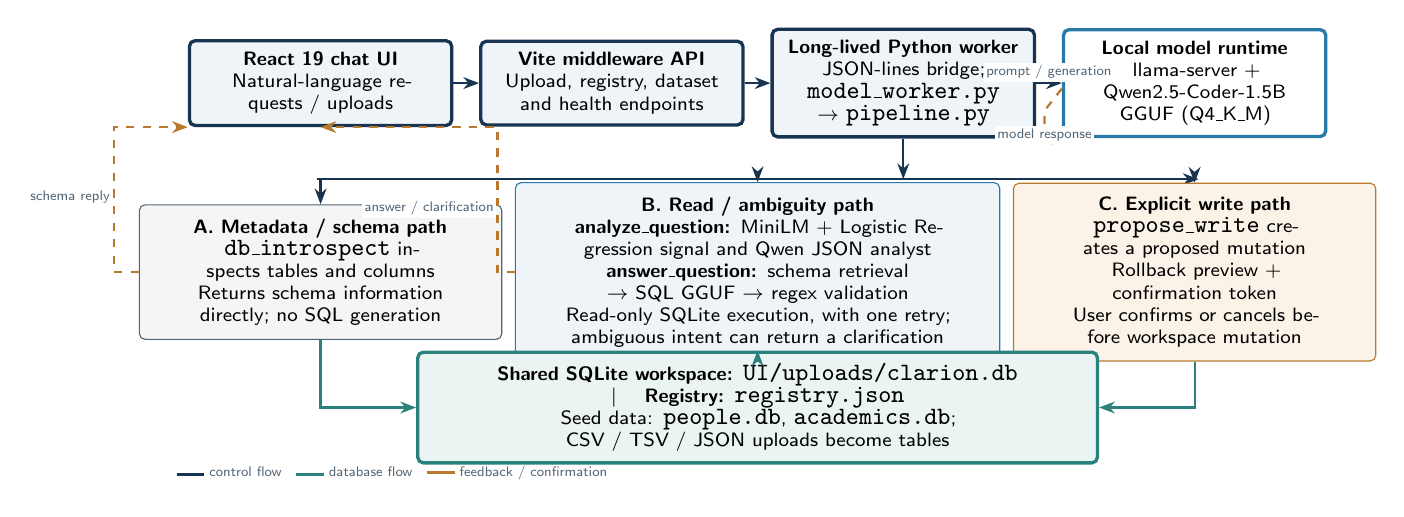
\begin{tikzpicture}[
  font=\sffamily\scriptsize,
  main/.style={draw=navy,very thick,rounded corners=2pt,fill=pale,align=center,minimum height=0.62cm,text width=3.05cm,inner sep=4pt},
  model/.style={draw=blue,very thick,rounded corners=2pt,fill=white,align=center,minimum height=0.62cm,text width=3.05cm,inner sep=4pt},
  store/.style={draw=teal,very thick,rounded corners=2pt,fill=tealpale,align=center,minimum height=0.62cm,text width=8.35cm,inner sep=4pt},
  meta/.style={draw=slate,rounded corners=2pt,fill=lightgray,align=center,text width=4.25cm,minimum height=1.18cm,inner sep=5pt},
  read/.style={draw=blue,rounded corners=2pt,fill=pale,align=center,text width=5.80cm,minimum height=1.46cm,inner sep=5pt},
  write/.style={draw=amber,rounded corners=2pt,fill=amberpale,align=center,text width=4.25cm,minimum height=1.18cm,inner sep=5pt},
  flow/.style={-{Stealth[length=2mm]},draw=navy,thick},
  dataflow/.style={-{Stealth[length=2mm]},draw=teal,thick},
  feedback/.style={-{Stealth[length=2mm]},draw=amber,dashed,thick},
  label/.style={font=\tiny\sffamily\color{slate},fill=white,inner sep=1pt}
]
% Runtime: UI -> API -> worker <-> model server
\node[main] (ui) at (0,0) {\textbf{React 19 chat UI}\\Natural-language requests / uploads};
\node[main] (api) at (3.70,0) {\textbf{Vite middleware API}\\Upload, registry, dataset and health endpoints};
\node[main] (worker) at (7.40,0) {\textbf{Long-lived Python worker}\\JSON-lines bridge; \code{model\_worker.py} $\rightarrow$ \code{pipeline.py}};
\node[model] (llama) at (11.10,0) {\textbf{Local model runtime}\\llama-server + Qwen2.5-Coder-1.5B GGUF (Q4\_K\_M)};
\draw[flow] (ui.east) -- (api.west);
\draw[flow] (api.east) -- (worker.west);
\draw[flow] (worker.east) -- node[label,above]{prompt / generation} (llama.west);
\draw[feedback] ([yshift=-2pt]llama.west) -- ++(-0.22,-0.28) |- node[label,pos=0.25,below]{model response} (worker.south east);

% Request router and three branches. The branch bus sits in clear space
% between the runtime row and the three request-path cards.
\coordinate (busL) at (-0.05,-1.22);
\coordinate (busR) at (11.15,-1.22);
\draw[flow] (worker.south) -- (7.40,-0.72) -- (7.40,-1.22);
\draw[flow] (busL) -- (busR);
\node[meta] (metadata) at (0.00,-2.40) {\textbf{A. Metadata / schema path}\\\code{db\_introspect} inspects tables and columns\\Returns schema information directly; no SQL generation};
\node[read] (readpath) at (5.55,-2.40) {\textbf{B. Read / ambiguity path}\\\textbf{analyze\_question:} MiniLM + Logistic Regression signal and Qwen JSON analyst\\\textbf{answer\_question:} schema retrieval $\rightarrow$ SQL GGUF $\rightarrow$ regex validation\\Read-only SQLite execution, with one retry; ambiguous intent can return a clarification};
\node[write] (writepath) at (11.10,-2.40) {\textbf{C. Explicit write path}\\\code{propose\_write} creates a proposed mutation\\Rollback preview + confirmation token\\User confirms or cancels before workspace mutation};
\draw[flow] (0.00,-1.22) -- (metadata.north);
\draw[flow] (5.55,-1.22) -- (readpath.north);
\draw[flow] (11.10,-1.22) -- (writepath.north);

% Shared workspace underneath all three paths
\node[store] (db) at (5.55,-4.12) {\textbf{Shared SQLite workspace:} \code{UI/uploads/clarion.db} \quad $\vert$ \quad \textbf{Registry:} \code{registry.json}\\Seed data: \code{people.db}, \code{academics.db}; CSV / TSV / JSON uploads become tables};
\draw[dataflow] (metadata.south) -- ++(0,-0.27) |- (db.west);
\draw[dataflow] (readpath.south) -- (db.north);
\draw[dataflow] (writepath.south) -- ++(0,-0.27) |- (db.east);
\draw[feedback] (metadata.west) -- ++(-0.32,0) |- node[label,pos=0.26,left]{schema reply} (ui.south west);
\draw[feedback] (readpath.west) -- ++(-0.22,0) |- node[label,pos=0.22,left]{answer / clarification} (ui.south);

% Legend
\node[font=\tiny\sffamily,anchor=west,text=slate] at (-1.95,-4.95) {\textcolor{navy}{\rule{0.35cm}{1.2pt}} control flow\quad \textcolor{teal}{\rule{0.35cm}{1.2pt}} database flow\quad \textcolor{amber}{\rule[1pt]{0.35cm}{1pt}} feedback / confirmation};
\end{tikzpicture}
\end{center}
\vspace{-2pt}
{\footnotesize\color{slate}\textbf{Figure 1.} Current Clarion runtime and its three request paths. The figure describes the supplied project audit; it does not imply that every component is production-hardened.}

\section{What happens to a request}
\begin{enumerate}[leftmargin=1.45em,label=\textcolor{blue}{\bfseries\arabic*.}]
  \item \textbf{Ingest and register.} CSV, TSV, and JSON uploads are converted into tables in a shared SQLite workspace; a registry tracks available datasets. The project also seeds the workspace from local SQLite fixtures.
  \item \textbf{Route by request type.} Schema/metadata questions use \code{db\_introspect}. Ordinary questions enter \code{analyze\_question}. Explicit mutations enter \code{propose\_write}.
  \item \textbf{Read and clarify.} The read path combines a MiniLM/Logistic Regression classifier signal with a Qwen JSON analysis, retrieves schema context, generates SQL, validates it, and executes against a read-only SQLite connection. A clarification is returned when the intent is not sufficiently resolved.
  \item \textbf{Preview writes.} Write requests are proposed first, previewed through a rollback flow, and associated with a confirmation token. The user can confirm or cancel before the mutation is applied.
\end{enumerate}

\vspace{1pt}
\begin{tabularx}{\linewidth}{>{\bfseries\color{navy}}p{2.15cm} X}
\toprule
Capability & Current implementation detail \\
\midrule
Data inputs & CSV / TSV / JSON ingestion into a SQLite workspace; seeded SQLite datasets are also present. \\
Read path & Question analysis, schema retrieval, SQL generation, regex validation, read-only execution, and one retry. \\
Write path & Explicit write proposal, rollback preview, token-based confirm/cancel flow. \\
Runtime & React 19, Vite middleware API, persistent Python worker, llama.cpp server, Qwen2.5-Coder-1.5B Q4\_K\_M model. \\
\bottomrule
\end{tabularx}

\vspace{5pt}
\colorbox{pale}{\parbox{\dimexpr\linewidth-2\fboxsep\relax}{\small
\textbf{Research framing.} Ambiguity detection and clarification are established research topics. Clarion's testable question is whether a small, schema-conditioned classifier can selectively coordinate with a local SLM to improve the accuracy--latency--resource trade-off across unseen user databases.\\[-1pt]
\textbf{Evaluation focus.} Macro-F1, per-class recall, false-clarification rate, clarification resolution, SQL execution accuracy, cross-schema generalization, end-to-end latency, and peak RAM.}}

\newpage
% ================================ PAGE 2 =====================================
{\color{navy}\sffamily\LARGE\bfseries Method, Evaluation and Current Status\par}
\vspace{2pt}
{\color{slate}\small A candid snapshot of what is implemented, what is measured, and what remains to be validated.}

\section{Ambiguity-aware decision method}
The intended method is to use a lightweight discriminative model for a first-pass signal and a compact language model for contextual interpretation. The database schema is part of the input: the same phrase can be clear in one schema and ambiguous in another.

\begin{center}
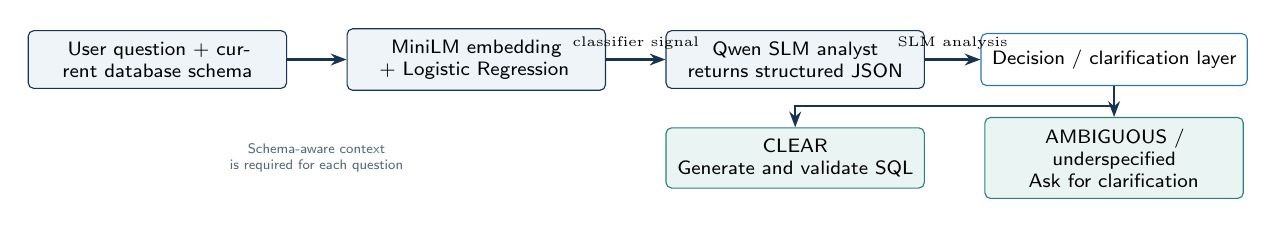
\begin{tikzpicture}[
  font=\sffamily\scriptsize,
  box/.style={draw=navy,rounded corners=2pt,fill=pale,align=center,text width=3.0cm,minimum height=0.66cm,inner sep=4pt},
  decision/.style={draw=blue,rounded corners=2pt,fill=white,align=center,text width=3.1cm,minimum height=0.66cm,inner sep=4pt},
  outbox/.style={draw=teal,rounded corners=2pt,fill=tealpale,align=center,text width=3.0cm,minimum height=0.72cm,inner sep=4pt},
  arr/.style={-{Stealth[length=2mm]},thick,draw=navy}
]
\node[box] (q) at (0,0) {User question + current database schema};
\node[box] (clf) at (4.05,0) {MiniLM embedding + Logistic Regression};
\node[box] (slm) at (8.10,0) {Qwen SLM analyst returns structured JSON};
\node[decision] (fuse) at (12.15,0) {Decision / clarification layer};
\draw[arr] (q) -- (clf);
\draw[arr] (clf) -- node[above,font=\tiny]{classifier signal} (slm);
\draw[arr] (slm) -- node[above,font=\tiny]{SLM analysis} (fuse);
\node[outbox] (clear) at (8.10,-1.25) {CLEAR\\Generate and validate SQL};
\node[outbox] (ask) at (12.15,-1.25) {AMBIGUOUS / underspecified\\Ask for clarification};
\draw[arr] (fuse.south) -- ++(0,-0.25) -| (clear.north);
\draw[arr] (fuse.south) -- (ask.north);
\node[font=\tiny\sffamily\color{slate},align=center] at (2.02,-1.25) {Schema-aware context\\is required for each question};
\end{tikzpicture}
\end{center}

\colorbox{redpale}{\parbox{\dimexpr\linewidth-2\fboxsep\relax}{\small
\textbf{Important implementation caveat.} The current fusion routine is not yet a genuinely balanced hybrid: when both classifier and SLM outputs are present, the selected decision follows the SLM label in the audited branches. The classifier therefore does not currently act as an effective veto or calibrated gate. The diagram above shows the intended component roles, not a claim that the fusion policy is already correct.}}

\section{Measured prototype status}
\begin{tabularx}{\linewidth}{>{\bfseries\color{navy}}p{2.65cm} >{\RaggedRight\arraybackslash}p{2.55cm} X}
\toprule
Measure & Observed value & Interpretation / limitation \\
\midrule
Classifier & 525 examples; 55.45\% held-out; 54.2\% unseen-schema & Weak performance; current model is not reliable enough to act as a standalone ambiguity gate. \\
Automated tests & 26 passed / 5 failed & The audited suite is red; safety-path tests need to be restored and rerun. \\
End-to-end SQL accuracy & Not established & The prior 30-pair score used a mismatched model/prompt path and inconsistent grading; do not quote it as a validated headline result. \\
Latency / peak RAM & Not established here & Measure the full served pipeline on fixed hardware; generation-only timing is insufficient. \\
\bottomrule
\end{tabularx}

\section{Current limitations and next engineering steps}
\begin{tabularx}{\linewidth}{>{\bfseries\color{navy}}p{2.45cm} X}
\toprule
Priority & Required improvement \\
\midrule
P0 -- decision quality & Fix classifier/SLM fusion; put the question before schema text; prevent schema truncation; calibrate thresholds on held-out data. \\
P0 -- correctness & Restore failing tests; evaluate the exact served model with the production schema builder and documented result normalization; expand database-level holdouts. \\
P1 -- SQL safety & Replace regex-only validation with SQLGlot parsing, one-statement enforcement, table/column checks, and read/write allowlists. Keep read-only SQLite and an authorizer as defense in depth. \\
P1 -- performance & Cache schema metadata; avoid repeated per-column value scans; bound prompt context; measure end-to-end latency and resource use. \\
P1 -- write UX / deployment & Show before/after diffs and re-check preview state at confirmation; separate the API from Vite dev mode before LAN use; add auth/origin checks, WAL/busy timeout, a write queue, and process shutdown. \\
\bottomrule
\end{tabularx}

\section{Selected related work}
\begin{multicols}{2}
\scriptsize
\textbf{Ambiguity benchmark.} A. Bhaskar, T. Tomar, A. Sathe, and S. Sarawagi, ``Benchmarking and Improving Text-to-SQL Generation under Ambiguity,'' EMNLP 2023, pp. 7053--7074.\newline
\url{https://aclanthology.org/2023.emnlp-main.436/}

\textbf{Conversational ambiguity.} M. Dong et al., ``PRACTIQ: A Practical Conversational Text-to-SQL Dataset with Ambiguous and Unanswerable Queries,'' NAACL 2025, pp. 255--273.\newline
\url{https://aclanthology.org/2025.naacl-long.13/}

\columnbreak
\textbf{Interactive disambiguation.} ``CLEAR: A Parser-Independent Disambiguation Framework for NL2SQL,'' IEEE ICDE 2025, DOI: 10.1109/ICDE65448.2025.00247.\newline
\url{https://ieeexplore.ieee.org/document/11113237/}

\textbf{Execution-grounded intent probing.} Y. Yin et al., ``Probing Ambiguity: Adversarial Intent Resolution for Robust Text-to-SQL,'' EMNLP 2026.\newline
\url{https://aclanthology.org/2026.emnlp-main.2446/}
\end{multicols}


\end{document}
